\documentclass[10pt]{elegantnote}
\usepackage{graphicx}
\usepackage{unicode-math}
\usepackage{framed} %段落加边框
\usepackage{makecell} %表格内强制换行
\usepackage{titletoc} % 章节目录
\usepackage{tabularx}
\usepackage{array}
\setmathfont{XITS Math}

% 取消pdf的压缩，最终版取消这个命令即可
\special{dvipdfmx:config z 0}

%自定义命令 颜色
\definecolor{epubblue}{RGB}{1,126,218}
\newcommand*{\cepubblue}{\textcolor{epubblue}}

% 字体

\RequirePackage[fontset=none]{ctex}
\setmainfont{Times New Roman}
\setCJKmainfont{SimSun}[BoldFont=FandolSong Bold, AutoFakeSlant]
\setCJKsansfont[BoldFont={FZHei-B01}]{FZKai-Z03}
\setCJKmonofont[BoldFont={FZHei-B01}]{FZFangSong-Z02}
\setCJKfamilyfont{zhsong}{FZShuSong-Z01}
\setCJKfamilyfont{zhhei}{FZHei-B01}
\setCJKfamilyfont{zhkai}[AutoFakeBold]{FZKai-Z03}
\setCJKfamilyfont{zhfs}[BoldFont={FZHei-B01}]{FZFangSong-Z02}
\setCJKfamilyfont{yahei}{Microsoft YaHei}
\setmathfont{XITS Math}

% 代码
\RequirePackage{listings}
%Python代码排版设置
\lstset{
    language=Python, % 设置语言
 breaklines=true, % 自动换行
 backgroundcolor=\color[rgb]{0.96,0.96,0.96},% 背景颜色
 keywordstyle=\bfseries\color{RoyalBlue}, % 设置关键字为粗体，颜色为 RoyalBlue
 morekeywords={}, % 设置更多的关键字，用逗号分隔
 emph={left,right,mid}, % 指定强调词，如果有多个，用逗号隔开
    emphstyle=\bfseries\color{Rhodamine}, % 强调词样式设置
    commentstyle=\color{black!50!white}, % 设置注释样式，斜体，浅灰色
    stringstyle=\color{PineGreen!90!black}, % 设置字符串样式
    columns=flexible,
    numbers=left, % 显示行号在左边
    numbersep=2em, % 设置行号的具体位置
    numberstyle=\footnotesize, % 缩小行号
    xleftmargin=1em, % 左边距
    xrightmargin=1em, % 右边距
    aboveskip=1em, % 上边距
    % framexleftmargin=2em, % 行号在框内
    framesep=1em, % 设置边框与代码的距离
    frame=shadowbox,rulesep=3pt,rulesepcolor=\color{red!20!green!20!blue!20} % 阴影边框
    }


\setlist[itemize,1]{\textcolor{ecolor}{\label=\bullet} }
\setlist[itemize,2]{\textcolor{ecolor}{\label=$\circ$} }

\begin{document}

\begin{sloppypar} %文字溢出自动换行


\begin{center}
    \bfseries \Large \textcolor{ecolor} {《程序语言设计》教学设计}

    \bfseries \Large \textcolor{ecolor} {张斌}
\end{center}

\tableofcontents

\newpage

\section{课程教学目标}
    \begin{enumerate}
        \item 掌握程序设计的基本知识和结构化编程的思想和方法；        
        \item 具备初步的程序设计能力，能够灵活运用模块化思想将复杂问题逐步分解，并且编写出相应的程序解决问题；
        \item 能够借助AI编写较为复杂的程序。
\end{enumerate}

\section{教学内容}

\subsection{安装Python环境与编辑器}

\subsubsection{安装Python}

    \begin{enumerate}
      \item 官网下载 https://www.python.org/downloads/windows/
      \item 安装
      \item 运行
      
      安装完成之后，进入命令行，输入python，正常情况下，会显示python的版本，就是安装成功了。
    \end{enumerate}

\subsubsection{配置编辑器}

    \begin{enumerate}
      \item 下载VSCode https://code.visualstudio.com/
      \item 安装VSCode
      \item 安装中文语言包
      \item 安装python插件
      \item 安装flake8(Python静态代码检查工具)和 yapf(python代码格式化工具)
        \begin{itemize}
          \item 打开命令行（cmd），按照下面的安装步骤：
          \item 输入pip3 list，检查是否已存在需要的包
          \item 继续输入pip3 install flake8，下载安装 flake8
          \item 继续输入pip3 install yapf，下载安装 yapf
        \end{itemize}
      \item 配置VS Code
        \begin{itemize}
          \item 左下角齿轮 > 设置 > 打开设置
          \item 在里面添加下面的代码：
          
          \begin{lstlisting}
            {
                "python.linting.flake8Enabled": true,
                "python.formatting.provider": "yapf",
                "python.linting.flake8Args": ["--max-line-length=248"], # 设置单行最长字符限制
                "python.linting.pylintEnabled": false # 关闭pylint工具
            }
          \end{lstlisting}
          \item 在VS Code中，按下快捷键 Alt+Shift+F 即可自动格式化代码。
        \end{itemize}
    \end{enumerate}

\subsection{变量/运算符}
\subsubsection{变量}
\begin{enumerate}
  \item 变量和类型
  \item 变量命名
  \item 变量的使用
\end{enumerate}
\subsubsection{运算符}
\begin{enumerate}
  \item Python中的运算符
  \item 算术运算符
  \item 赋值运算符
  \item 比较运算符
  \item 逻辑运算符
\end{enumerate}

\subsection{程序的结构}

程序的三种基本结构：顺序结构，分支结构，循环结构。

Python中使用缩进的方式来表示代码的层次结构，缩进可以使用任意数量的空格，但通常使用4个空格。

\subsubsection{顺序结构}
一条一条语句顺序执行，这种代码结构通常称之为顺序结构。然而仅有顺序结构并不能解决所有的问题。
\subsubsection{分支结构}
    \begin{itemize}
      \item 利用if、elif和else构建分支结构
      \item 注意if、elif和else的最后面有一个冒号:
      \item 连续的代码保持相同的缩进那么它们属于同一个代码块
    \end{itemize}

    \begin{lstlisting}
        score = float(input('请输入成绩: '))
        if score >= 90:
            grade = 'A'
        elif score >= 80:
            grade = 'B'
        elif score >= 70:
            grade = 'C'
        elif score >= 60:
            grade = 'D'
        else:
            grade = 'E'
        print('对应的等级是:', grade)
    \end{lstlisting}
\subsubsection{循环结构}
    \begin{itemize}
      \item for-in循环
      
      \begin{lstlisting}
        # 1到100的和
        total = 0
        for x in range(1, 101):
            total += x
        print(total)
      \end{lstlisting}
      \item while循环
      
      \begin{lstlisting}
        # 1到100的和
        total = 0
        x = 1
        while x <= 100:
            total += x
            x += 1
        print(total)
      \end{lstlisting}
      \item 结束循环
      \item 循环结构嵌套
      
      \begin{lstlisting}
        # 九九乘法表
        for i in range(1, 10):
        for j in range(1, i + 1):
            print(f'{i}*{j}={i * j}', end='\t')
        print()
      \end{lstlisting}
    \end{itemize}

\subsection{数据结构}


\subsubsection{字符串}
    \begin{itemize}
      \item 定义
      \item 转义字符
      \item 字符串的运算
        \begin{itemize}
          \item 拼接
          \item 比较
          \item 成员
          \item 长度
          \item 索引和切片
          \item 循环遍历
        \end{itemize}
      \item 字符串的方法
        \begin{itemize}
          \item 大小写
          \item 查找
          \item 格式化
          \item 修剪
          \item 替换
          \item 拆分/合并
        \end{itemize}
    \end{itemize}
\subsubsection{列表}
    \begin{itemize}
      \item 定义和使用列表
      \item 列表的运算符
      \item 列表元素的遍历
      \item 嵌套列表
      \item 操作列表
      \begin{itemize}
        \item 添加和删除元素
        \item 查找元素位置
        \item 元素排序和反转
        \item 列表的生成式
      \end{itemize}
    \end{itemize}
\subsubsection{字典}
    \begin{itemize}
      \item 创建和使用字典
        \begin{itemize}
          \item 创建空字典
          \item 访问字典里的值
          \item 修改字典
          \item 删除字典元素
        \end{itemize}
      \item 字典的运算
        \begin{itemize}
          \item 成员运算
          \item 索引运算
        \end{itemize}
      \item 字典的方法
        \begin{itemize}
          \item 返回指定键的值
          \item 删除键所对应的值
          \item 获取字典中所有的键值对
          \item 对字典中所有的键值对进行循环遍历
          \item 更新字典元素
        \end{itemize}
    \end{itemize}

\subsection{函数}

函数是组织好的，可重复使用的，用来实现单一，或相关联功能的代码段。函数能提高应用的模块性，和代码的重复利用率。你已经知道Python提供了许多内建函数，比如print()。但你也可以自己创建函数，这被叫做用户自定义函数。

\subsubsection{定义函数}

在Python中可以使用def关键字来定义函数，和变量一样每个函数也应该有一个漂亮的名字，命名规则跟变量的命名规则是一致的。在函数名后面的圆括号中可以放置传递给函数的参数。

函数的基本语法如下所示：

\begin{lstlisting}
def function_name():
    # What you want the function to do
\end{lstlisting}

一个函数示例如下所示：
\begin{lstlisting}
def learn_to_code():
    print("I like coding.")
\end{lstlisting}

这个函数做的是打印文本“I like coding.”到终端。函数不只能实现打印功能，还可以通过return关键字来返回函数的执行结果。

\subsubsection{函数调用}

\subsubsection{函数的参数}
    \begin{itemize}
      \item 必需参数
      \item 关键字参数
      \item 默认参数
    \end{itemize}

指出下面的代码中的错误：
\begin{lstlisting}
def describe_pet(pet_name='willie', animal_type):
    print(f"\nI have a {animal_ type}.")
    print(f"My {animal_ type}'s name is {pet_name.title()}.")

describe_pet(animal_type='dog')
\end{lstlisting}

使用 默认值 时， 必须 先在 形 参 列表 中 列出 没有 默认值 的 形 参， 再 列出 有 默认值 的 实 参。 这 让 Python 依然 能够 正确地 解读 位置 实 参。

    \subsubsection{模块}
    \begin{itemize}
      \item random随机数模块
      \item time时间模块
      \item os模块
      \item os.path 系统路径操作
      \item pandas 数据分析
    \end{itemize}

\subsubsection{在AI的帮助下做一个点名程序}

{\bfseries 通过此示例程序，理解函数的功能。}

\begin{framed}
    我的班级里有10个学生，希望你能用python做一个带GUI的程序实现点名功能，这个程序会滚动随机显示学生姓名，当按下按钮后停止。
\end{framed}

询问chatGPT，给出如下程序：

\begin{lstlisting}
import tkinter as tk
import random

class RollCallApp:
    def __init__(self, students):
        self.students = students
        self.current_student = ""
        self.roll_call_running = False
        self.root = tk.Tk()
        self.label = tk.Label(self.root, text="")
        self.button = tk.Button(self.root, text="开始点名", command=self.toggle_roll_call)
        self.label.pack()
        self.button.pack()

    def toggle_roll_call(self):
        if self.roll_call_running:
            self.stop_roll_call()
        else:
            self.start_roll_call()

    def start_roll_call(self):
        if not self.roll_call_running:
            self.roll_call_running = True
            self.roll_call()

    def stop_roll_call(self):
        self.roll_call_running = False

    def roll_call(self):
        if self.roll_call_running:
            self.current_student = random.choice(self.students)
            self.label.config(text=self.current_student)
            self.label.after(200, self.roll_call)
        else:
            self.label.config(text=self.current_student)

    def run(self):
        self.root.mainloop()

# 学生名单
students = ["学生1", "学生2", "学生3", "学生4", "学生5", "学生6", "学生7", "学生8", "学生9", "学生10"]

app = RollCallApp(students)
app.run()
\end{lstlisting}

\begin{framed}
    我们可以用Tkinter库创建一个带有GUI的点名程序。

    在这个示例中，我们创建了一个名为RollCallApp的类，它包含一个学生名单和一个基于Tkinter的GUI窗口。在初始化方法中，我们创建了一个标签和一个按钮，并将它们放置在窗口中。当点击按钮时，\verb|roll_call|方法会从学生名单中随机选择一个学生，并在标签上显示其姓名。

    \verb|self.current_student|和\verb|self.roll_call_running|两个变量用来跟踪当前显示的学生姓名和点名状态。在\verb|start_roll_call|方法中，我添加了一个条件判断，确保只有当点名没有在进行时才能启动点名。

    

    \verb|toggle_roll_call|方法用于切换点名状态，当点名正在进行时，点击按钮会停止点名；当点名没有在进行时，点击按钮会开始点名。

在\verb|stop_roll_call|方法中，我们将\verb|roll_call_running|变量设置为False，表示停止点名。

在\verb|roll_call|方法中，如果点名正在进行，它会继续更新学生姓名并进行滚动；如果点名已停止，它会将最终的学生姓名显示在标签上。

在\verb|roll_call|方法中，我使用after方法将\verb|roll_call|方法自身以一定的时间间隔（这里设置为200毫秒）添加到Tkinter事件队列中。这样就可以实现在每个时间间隔内刷新学生姓名并实现滚动的效果。

    当点击"开始点名"按钮时，点名程序开始执行，并以滚动的方式显示学生姓名。再次点击按钮可以停止点名。

    你可以根据需要修改学生名单或进行其他自定义调整。运行代码后，将弹出一个窗口，点击"点名"按钮时，窗口中的标签将会显示一个随机选择的学生姓名。

    请注意，这只是一个简单的示例程序，你可以根据自己的需求进一步扩展和美化GUI界面。
\end{framed}

{\bfseries 请你对点名程序做如下修改：}

\begin{enumerate}
  \item 将学生名单更改为自己班的名单
  \item 将滚动时间改为0.1秒
  \item 更改窗口大小和文字颜色大小
\end{enumerate}

更改前：
\begin{figure}[htpb]
    \centering
    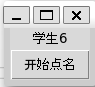
\includegraphics{点名}
\end{figure}

更改后效果：
\begin{figure}[htpb]
    \centering
    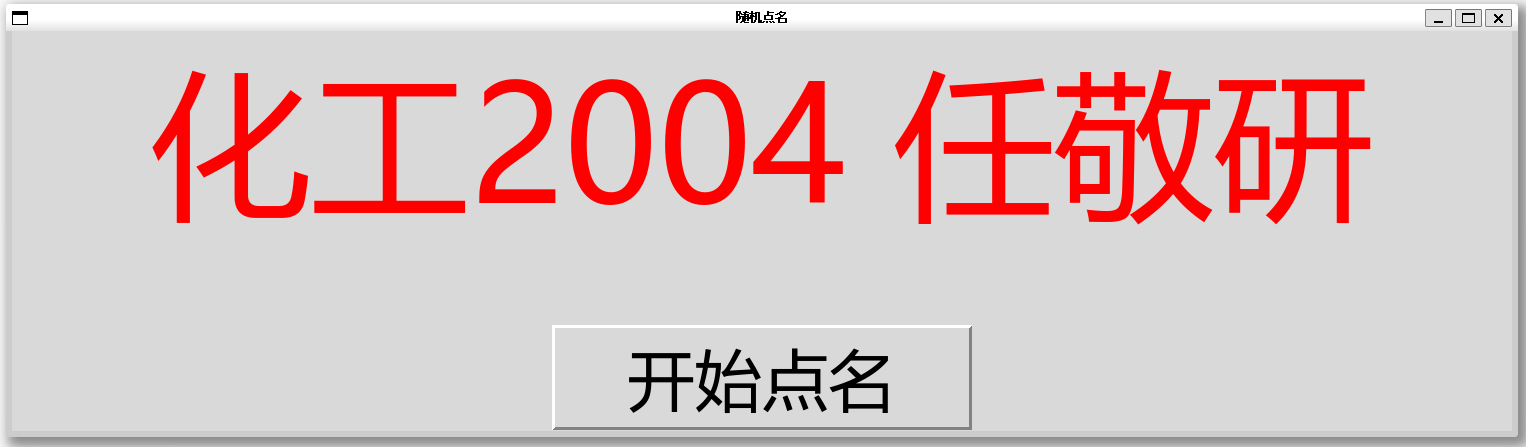
\includegraphics[width=\linewidth]{点名2}
\end{figure}


\subsection{读写excel文件}

openpyxl：主要针对xlsx格式的excel进行读取和编辑，简单易用，功能广泛。

pandas：数据处理最常用的分析库之一，可以读取各种各样格式的数据文件，一般输出dataframe格式，功能强大。

安装：

\begin{lstlisting}
pip install openpyxl
pip install pandas
\end{lstlisting}



\subsubsection{读取Excel文件}

要加载一个已存在的 Excel 文件，需要用 \verb|load_workbook| 方法，给定文件路径，返回 workbook 对象：

\begin{lstlisting}
from openpyxl import load_workbook

wb = load_workbook('test.xlsx')

# 显示文档中包含的 表单 名称
print(wb.sheetnames)
\end{lstlisting}

workbook 相当于一个 Excel 文件档，每个被创建和打开的 Excel 文件都是独立的 Workbook 对象。

\subsubsection{写入Excel文件}

\begin{lstlisting}
from openpyxl import Workbook
# 创建一个 workbook
wb = Workbook()
# 获取被激活的 worksheet
ws = wb.active
# 设置单元格内容
ws['A1'] = 42
# 设置一行内容
ws.append([1, 2, 3])
# python 数据类型可以被自动转换
import datetime
ws['A2'] = datetime.datetime.now()
# 保存 Excel 文件
wb.save("sample.xlsx")
\end{lstlisting}

结果如图：

\begin{figure}[htpb]
    \centering
    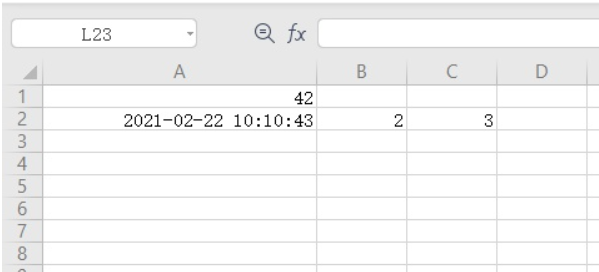
\includegraphics[width=.6\linewidth]{excel}
\end{figure}

\subsubsection{合并多个数据格式相同的Excel文件}

\begin{lstlisting}
import os,time
import pandas as pd
start_time=time.time()
dir = r'D:\合并excel' # 设置工作路径

# 新建列表，存放每个文件数据框（每一个excel读取后存放在数据框,依次读取多个相同结构的Excel文件并创建DataFrame）
DFs = []

for root, dirs, files in os.walk(dir):  # 第一个为起始路径，第二个为起始路径下的文件夹，第三个是起始路径下的文件。
    for file in files:
        file_path=os.path.join(root,file)  # 将路径名和文件名组合成一个完整路径
        df = pd.read_excel(file_path) # excel转换成DataFrame
        DFs.append(df)
# 合并所有数据，将多个DataFrame合并为一个
alldata = pd.concat(DFs)  # sort='False'


alldata.to_excel(r'D:\合并excel\合并结果.xlsx',index = False)
end_time=time.time()
times=round(end_time-start_time,2)
print('合并完成，耗时{}秒'.format(times))
\end{lstlisting}


\subsection{借助AI解决复杂实际问题}

\subsubsection{答辩分组}

化工制药系2023届毕业生共285人，其中化工142人，制药143人。现在需要进行毕业答辩分组安排，共设5个答辩组，要求每个答辩组的学生随机分配，各个答辩组人数平均分配。

根据需求询问chatGPT，给出如下回答：

\begin{framed}
    班里有50名学生，10名老师，每个老师指导5个学生。现在需要对师生进行答辩安排，分成5个答辩组，每组2个老师，要求学生不能在指导老师所在的答辩组。请你根据指导老师-学生名单，设计一个python程序进行分组。
\end{framed}

\begin{lstlisting}
import random

# 指导老师和学生名单
teachers = ["Teacher1", "Teacher2", "Teacher3", "Teacher4", "Teacher5", "Teacher6", "Teacher7", "Teacher8", "Teacher9", "Teacher10"]
students = ["Student1", "Student2", "Student3", "Student4", "Student5", "Student6", "Student7", "Student8", "Student9", "Student10",
"Student11", "Student12", "Student13", "Student14", "Student15", "Student16", "Student17", "Student18", "Student19", "Student20",
"Student21", "Student22", "Student23", "Student24", "Student25", "Student26", "Student27", "Student28", "Student29", "Student30",
"Student31", "Student32", "Student33", "Student34", "Student35", "Student36", "Student37", "Student38", "Student39", "Student40",
"Student41", "Student42", "Student43", "Student44", "Student45", "Student46", "Student47", "Student48", "Student49", "Student50"]

# 随机排序学生名单和老师名单
random.shuffle(students)
random.shuffle(teachers)

# 每个答辩组的老师数量
teachers_per_group = 2

# 每个老师的指导学生数量
students_per_teacher = 5

# 计算答辩组的数量
num_groups = len(teachers) // teachers_per_group

# 分组字典，键为答辩组编号，值为对应答辩组的老师列表和学生列表
groups = {group_num: {"teachers": [], "students": []} for group_num in range(1, num_groups + 1)}

# 按老师的指导学生数量进行分组
for i in range(0, len(teachers), teachers_per_group):
    group_num = i // teachers_per_group + 1
    teacher_list = teachers[i:i + teachers_per_group]
    student_list = students[:teachers_per_group * students_per_teacher]
    students = students[teachers_per_group * students_per_teacher:]
    groups[group_num]["teachers"] = teacher_list
    groups[group_num]["students"] = student_list

# 检查学生是否在指导老师所在的组，并进行调整
for group_num, group_data in groups.items():
    teachers_in_group = group_data["teachers"]
    students_in_group = group_data["students"]
    for teacher in teachers_in_group:
        students_to_swap = []
        for student in students_in_group:
            if student in groups[group_num]["teachers"]:
                students_to_swap.append(student)
        for student in students_to_swap:
            students_in_group.remove(student)
            random_group_num = random.choice(list(groups.keys()))
            while student in groups[random_group_num]["teachers"] or student in groups[random_group_num]["students"]:
                random_group_num = random.choice(list(groups.keys()))
            groups[random_group_num]["students"].append(student)

# 输出分组结果

for group_num, group_data in groups.items():
    print(f"Group {group_num}:")
    print("Teachers:", group_data["teachers"])
    print("Students:", group_data["students"])
print()
\end{lstlisting}

\begin{framed}
    这个程序将学生和老师名单作为输入，通过随机排序学生和老师名单，然后按照每组包含2个老师的要求，将老师和学生进行分组，并确保学生不会在指导老师所在的组。

请注意，这个程序假设每个老师指导的学生数量是固定的，并且能够被答辩组数量整除，以确保每个老师和学生都能被分配到一个组。

你可以根据需要替换学生和老师的名单，然后运行程序以获取分组结果。
\end{framed}

{\bfseries 请根据指导教师-学生名单，以及答辩组教师安排名单，结合chatGPT给出的代码，编写一个程序，使其能够完成答辩分组的工作。如果你能将每组的化工/制药学生数量平均分配就更好了。

附件1：指导教师-学生名单

附件2：答辩组教师名单}

\subsubsection{文件重新分组}

化工制药系的毕业论文材料归档工作已经完成，每个专业一个文件夹，论文命名方式为学号-姓名-题目。目录结构如下：

\begin{verbatim}
|-论文终稿
| |  
| |-化工
| |  
| |    2018984060115-何志阳-年产10万吨环己酮（反应工段）的生产工艺设计.pdf
| |    2018984060213-袁泽超-年产5万吨丙烯腈生产工艺设计.pdf
| |    ......
| |    2019984060528-丁姿瑜-年产20万吨己二腈工艺生产设计.pdf
| |    2019985060529-陈鹤-年产5万吨戊醇的合成工段的工艺设计.pdf
| |  
| |-制药
| |    2017984030316-岳茜漫-年产2亿片格列本脲二甲双胍片生产工艺设计.pdf
| |    2019984030101-赵子辰-年产10亿片复方氨酚烷胺片工艺设计.pdf
| |    ......
| |    2019984030528-陈璐-年产10万吨盐酸苯达莫司汀生产工艺设计.pdf
| |    2019984030529-安晓红-年产100吨依折麦布生产工艺设计.pdf
\end{verbatim}

教务处要求对论文进行全面复审，化工制药系决定复审工作按答辩组进行。现在请根据上一节分配好的答辩组学生名单，将全部论文按答辩组重新归档，每个答辩组一个文件夹。

根据需求询问chatGPT，给出如下回答：

\begin{framed}
    我有一些文件，现在我想根据不同的关键字将这些文件移动到指定文件夹中，如何用python实现？
\end{framed}

\begin{lstlisting}
import os
import shutil

def move_files_with_keywords(source_folder, destination_folder, keywords):
    # 遍历源文件夹中的文件
    for root, dirs, files in os.walk(source_folder):
        for file in files:
            # 检查文件名是否包含关键字
            if any(keyword in file for keyword in keywords):
                # 构建源文件路径和目标文件路径
                source_path = os.path.join(root, file)
                destination_path = os.path.join(destination_folder, file)
                # 移动文件到目标文件夹
                shutil.move(source_path, destination_path)
                print(f"Moved file: {file}")

# 指定源文件夹路径、目标文件夹路径和关键字列表
source_folder = 'D:\\ source_folder'
destination_folder = 'D:\\ destination_folder'
keywords = ['example', 'keyword', 'test']

# 调用函数进行移动操作
move_files_with_keywords(source_folder, destination_folder, keywords)    
\end{lstlisting}

\begin{framed}
要使用Python实现将包含特定关键字的文件移动到指定文件夹，你可以使用os模块和shutil模块。

在上述代码中，关键字被存储在名为keywords的列表中。any(keyword in file for keyword in keywords)这个表达式将迭代关键字列表，并检查文件名是否包含其中任何一个关键字。如果文件名包含任何一个关键字，就会将该文件移动到目标文件夹中。

请确保根据实际情况修改代码中的源文件夹路径、目标文件夹路径和关键字列表。这样，包含任何一个关键字的文件都将被移动到指定的目标文件夹中。移动完成后，会在控制台输出被移动的文件名。
\end{framed}

{\bfseries 现在请你结合chatGPT给出的代码编写一个程序，使其能够完成对论文进行重新分组的工作。}

\end{sloppypar}
\end{document}